\section{Ganzzahlig-lineare Programmierung \skript{63}}
  \begin{minipage}{7cm}
    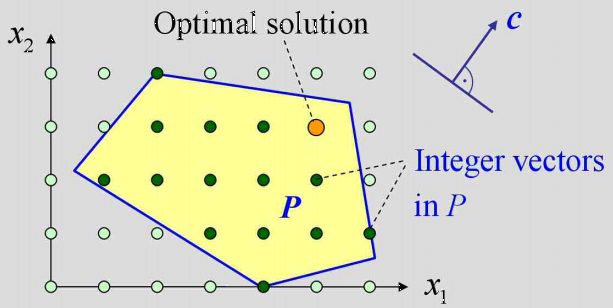
\includegraphics[width=7cm]{./Content/IntProg/intprog}
  \end{minipage}
  \begin{minipage}{12cm}
	  Als zusätzliche Nebenbedingung zu LP dürfen Variablen nur ganzzahlig (integer, ILP) sein, das macht das Problem einiges komplizierter.
	  Konkret sind LP polynomial lösbar, während ILP NP-vollständig (NP-complete) sind.
	    
  	\subsection{Relaxationen}
  		Um Schranken (obere/untere) zu berechnen, kann der \em Lösungsraum
  		vergrössert \em werden (Relaxationen). Beispiel: Der höchste Berg in
  		Tibet ist höchstens so gross wie der höchste Berg in China (China
  		$\rightarrow$ grösserer Lösungsraum als Tibet). In ILP wird \em
  		LP-Relaxation \em verwendet, d.h. die Ganzzahligkeitsforderung wird
  		fallen gelassen.
	\end{minipage}
  
		

\subsection{Branch-and-Bound Verfahren \skript{68}}
	\begin{minipage}{8cm}
		Um die optimale Lösung zu finden, wird das Lösungsgebiet aufgeteilt und jeweils sowohl eine obere als auch eine untere Schranke der Lösung gesucht. Falls die Schranken bereits eine optimale Lösung ausschliessen (wenn bei einem anderen Ast die untere Schranke höher ist als die obere beim aktuellen), kann die Suche innerhalb dieses Astes abgebrochen werden. Man spricht von \em Pruning by Dominance\em. Optimalität ist gefunden, wenn die obere gleich der unteren Schranke ist.
		
		Details für ILP: \skript{72f.}\\
		B\&B ist geeignet für beliebige Optimierungsprobleme (inkl. nichtlineare). Die Terminierung nach endlicher Anzahl Schritten ist jedoch nur bei endlichen Lösungsräumen gewährleistet.
	\end{minipage}
	\begin{minipage}{10cm}
		Beispiel: Helikopter $\Leftrightarrow$ Sherpas.
		
		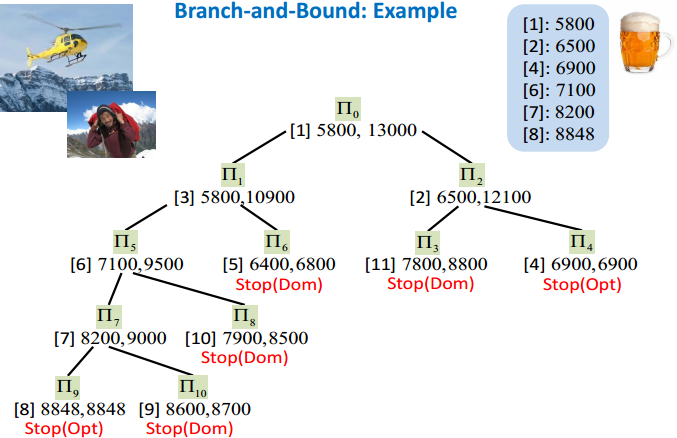
\includegraphics[width=10cm]{Content/IntProg/branch-bound}
	\end{minipage}
\subsubsection{Beispiel: Branch-and-bound beim Knapsack-Problem \skript{73--78}}

\textbf{Lower bound:}\\
Lower bound ist die global gespeicherte beste Item-Auswahl, die wir bis jetzt angetroffen haben und somit Kandidat für globales Optimum. (Vgl. 'Bar in Kathmandu')\\

\textbf{Upper bound:}\\
In einem beliebigen Knoten berechnet sich der upper bound wie folgt:
\begin{itemize}
	\item Items, für die im aktuellen Knoten noch keine Entscheidung getroffen wurde, sortieren nach $\frac{Wert}{Gewicht}$ ('Wertdichte').
	\item Soviele (ganze) Items einpacken wie Platz dafür vorhanden ist.
	\item Vom nächst'dichteren' einen Bruchteil einpacken, s.d. das maximale Gewicht ausgereizt ist. (LP-Relaxation)
	\item Mehr Wert kann in diesem Knoten nicht erreicht werden, somit handelt es sich um den upper bound.
	\item Wenn der upper bound kleiner ist, als was wir (global gespeichert) schon erreicht haben, können wir abbrechen. (\em pruning by dominance\em)
\end{itemize}

\textbf{Heuristische Lösungssuche:}\\
Packe von den noch nicht definitiv (ab)gewählten Elementen soviele (nach Wertdichte sortierte) ein, wie es dafür Platz im Rucksack hat. (ACHTUNG: Im Wurzelknoten hat es also typischerweise zu Beginn bereits mehr als ein Element im Rucksack.)\\

\textbf{Definition der Teilprobleme:}\\
Um aus einem Knoten die beiden Nachfolge-Knoten zu bilden wird wie folgt vorgegangen:
\begin{itemize}
	\item Dasjenige Element, das nur partiell Platz hatte im rechten Teilbaum definitv wählen und im linken definitiv abwählen.
	\item Die heuristische Lösungssuche neu durchführen.
\end{itemize}

\textbf{Strategie der Knotenwahl:}\\
Für die Wahl des nächsten zu expandierenden Knotens gibt es verschiedene Ansätze. Wir fahren eine Depth-first-search Strategie. Dazu expandieren wir immer den rechtesten Knoten, welcher noch nicht geprunt wurde.\\
 
\textbf{Arbeitsschritte:}
\begin{enumerate}
	\item Iterationsnummer inkrementieren und in eckigen Klammern notieren
	\item Zu expandierenden Knoten $r$ bestimmen (gemäss 'Strategie der Knotenwahl')
	\item Vorgänger-Knoten in Klammern notieren (falls vorhanden, sonst '.')
	\item Menge der definitiv abgewählten Knoten $J^0_r$ und definitiv gewählten Knoten $J^1_r$ notieren.
	\item Bitvektor-Auswahl für upper bound $x_r^{UB}=x^{LP}$ notieren (enthält Bruchteil von item)
	\item (Imaginären) Rucksackwert $z_r^{UB}=z^{LP}$ berechnen und auf pruning by dominance prüfen ($z_r^{UB}\le z^{LB}$) (bester bisher erreichter Wert kann sicher nicht erreicht werden); Falls pruning by dominance weiter mit Schritt 1.
	\item Bitvektor-Auswahl $x_r^{LB}$ notieren und zugehörigen Rucksackwert $z_r^{LB}$ berechnen
	\item Auf global update für lower bound $(z_r^{LB} > z^{LB})$ prüfen, ggf. updaten.
	\item Auf pruning by optimality $(z_r^{LB} = z^{UB})$ prüfen.
	\item Branching ausführen (Teilprobleme bilden)
	\item Weiter bei Schritt 1.
\end{enumerate}

\subsection{Schnittebenenverfahren (Cutting Planes) \skript{78}}  
	%\todo{RK: Keine Übungen dazu gefunden... ZF nötig??}
	
	Durch Linearkombination der Bedingungen, ist eine Einschränkung des Lösungsgebiets möglich. Die Multiplikatoren werden durch "pröbeln" gefunden. Beispiel:
	
	\begin{tabular}{p{8cm} p{4cm} p{3cm}}
		Ursprüngliche Bedingung 1 & $x_1 + 3 x_2 \leq 6$ & $| \cdot \frac{5}{8}$\\
		Ursprüngliche Bedingung 2 & $3 x_1 + x_2 \leq 6$ & $| \cdot \frac{1}{8}$  \\
		Aufsummiert: & $x_1 + 2 x_2 \leq \lfloor 4.5 \rfloor \overbrace{=}^{!} 4$ \\
	\end{tabular}
